\graphicspath{{./assets/}}

\section{Spule}
\subsection{Definition und Aufbau der Spule}
\begin{frame}
    \makeframetitle

    \begin{columns}
        \begin{column}{0.5\textwidth}
            \begin{itemize}
                \item Spiralförmig gewickelter Draht
                \item Passives Bauelemente
                \item \alert{Besondere Eigenschaft}: hohe \textit{Induktivität}
            \end{itemize}
        \end{column}
        \begin{column}{0.5\textwidth}
            \begin{figure}
                \centering
                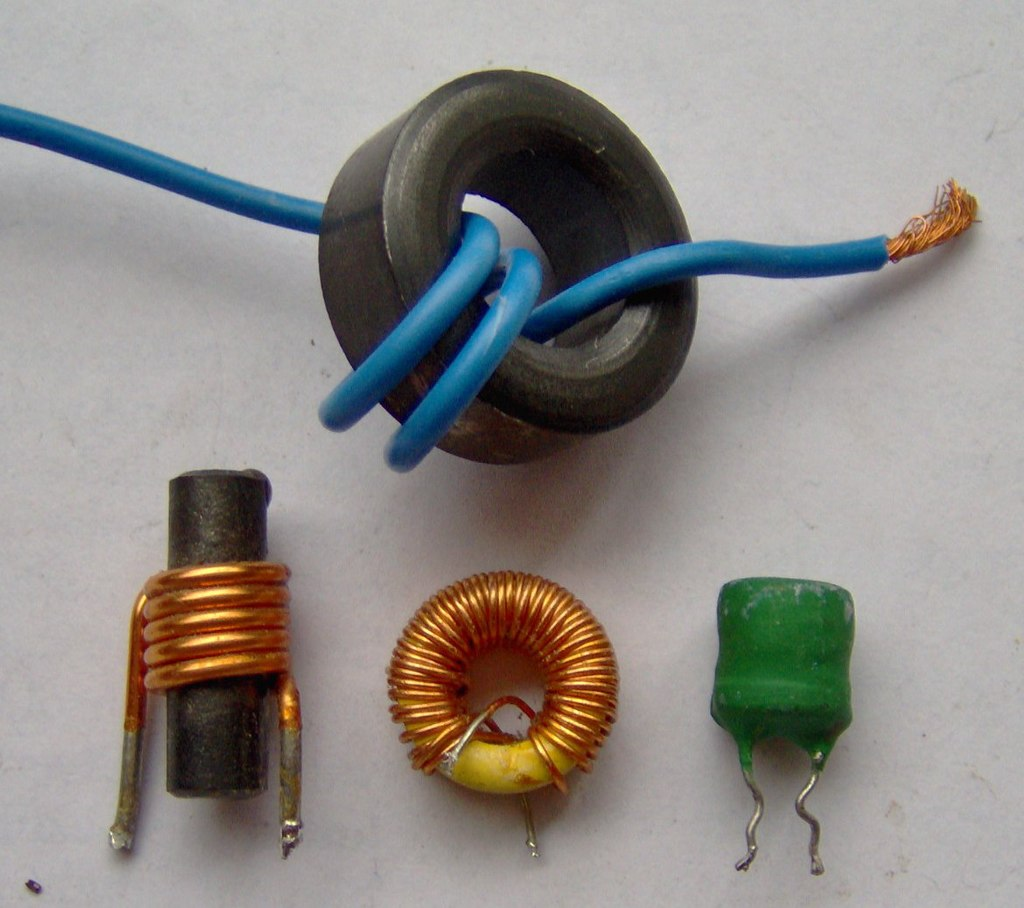
\includegraphics[width=0.8\textwidth]{Electronic_component_inductors}
                \caption{Bild einiger Spulen/Drosseln\cite{miguel_spule_2007}}
            \end{figure}
        \end{column}
    \end{columns}
        
\end{frame}

\begin{frame}
    \makeframetitle
    \begin{itemize}
        \item Meist um einen festen Körper gewickelt
        \item Die einzelnen Windungen müssen voneinander \textit{isoliert}
            sein
        \item Man spricht von einer \alert{Luftspule}, wenn der Wickelkörper
            \textit{nichtmagnetisch} ist
        \item Schaltzeichen der Spule: \\
            \begin{figure}
                \centering
                \begin{circuitikz}
                    \draw
                    (0, 2) to [american inductor, o-o] (0, 0)
                    ;
                \end{circuitikz}
                \caption{Schaltzeichen}
            \end{figure}
    \end{itemize}
\end{frame
